
\subsection{Simulation Results}

Corollaries \ref{cor: consequence of main theorem 1}, \ref{cor: consequence of main theorem 2}, and \ref{cor: consequence of main theorem 3} offer theoretical guidance on the optimal choice of $\lamz$ for minimizing the upper bound on excess risk. However, these results do not guarantee that the same value of $\lamz$ is optimal for the true excess risk. To explore this, we conduct simulations to empirically identify the value of $\lamz$ that minimizes the actual excess risk.

We conduct a simulation study to find the empirical distribution of the optimal regularization parameter, $\lamz$. We generate $100$ different distributions over $(X, Y, Z)$, each constructed as follows:

\begin{enumerate}
    \item The features $X$ are sampled from a Gaussain mixture model, whose parameters and mixing probabilities are randomly choosen.
    
    \item Then the weight vectors $u$ and $w$ are sampled from standard normal distribution.    
    Given fixed weights $u$, the binary variables $Z$ is sampled via logistic models:
    \[ Z \sim \sigma((1,X)^\top u).\]
    Once we get $Z$, then for a fixed weight $w$, the binary variable $Y$ is sample via logistic model:
    \[ Y \sim \sigma((1,X,Z)^\top w).\]
    
\end{enumerate}

This process is repeated $100$ times, each with a new random choice of parameters, resulting in a diverse family of distributions for evaluating the bang-bang behavior of the optimal $\lamz$.

For each distribution, we generate $m=1000$ samples for the $(X, Z)$ dataset (used for learning $X \to Z$), $n=4000$ samples for the $(X, Y)$ dataset (used for learning $X \times Z \to Y$), and $t=20000$ samples for the test set $(X, Y, Z)$ to compute the excess risk. 
For each value of $\lamz$ in the candidate set
\begin{equation*}
    \{0.01, 0.1, 1.0, 10.0, 100.0, 1000.0, 10000.0, 100000.0\},
\end{equation*}
a model is trained and evaluated. The optimal $\lamz$ for each distribtution is chosen as the value that yields the lowest empirical excess risk on the test set.

The frequency of each candidate $\lambda$ value being chosen as the optimal $\lamz$ across the $100$ distributions is shown in Figure \ref{fig: lambda plot}. The simulation results, summarized in the frequency plot, show a strong preference for the extreme values of the regularization parameter $\lamz$. This observed bang-bang behavior of $\lambda_z$ provides empirical evidence suggesting a bang-bang nature of $\lambda_z$.

\begin{figure}[htbp]
\centering
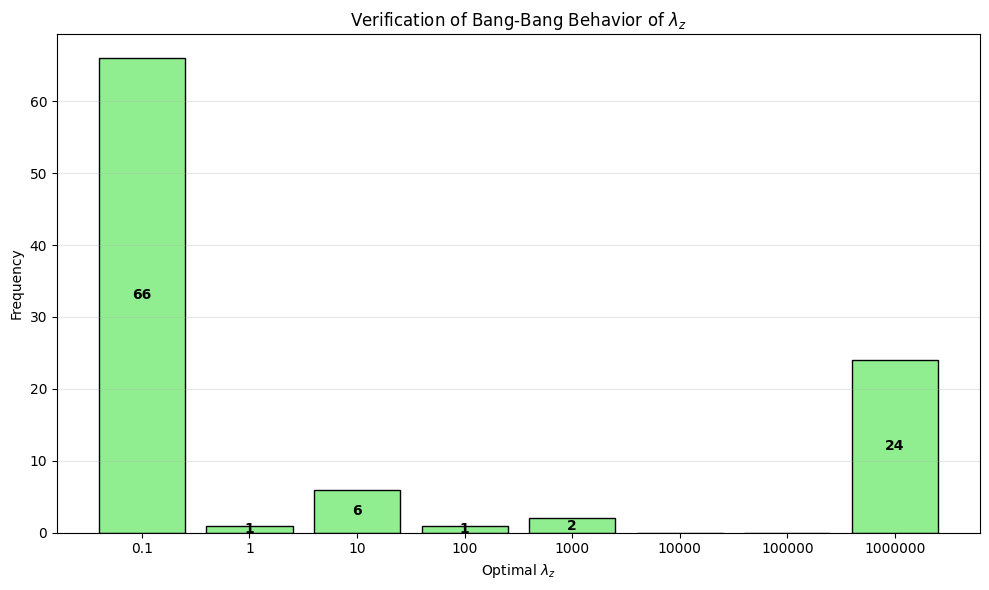
\includegraphics[scale=0.5]{lambda_frequency.png}

\caption{Frequency of optimal $\lamz$ values across 100 independent simulation seeds. For each seed, $\lamz$ is the value from the set $\{0.1, 1, 10, 100, 1000, 10000, 100000, 1000000\}$ that minimizes the empirical excess risk.}
\label{fig: lambda plot}

\end{figure}
\FloatBarrier




